\setcounter{figure}{8}
\section*{S17. Stable non-normal returns, innovation geometry, and gate calibration}
Run \texttt{python strengthen.py} to regenerate Supplementary Figures S9--S10. Numerical output is saved in \texttt{strengthening\_\allowbreak results.json}. S9 uses the exact matrix, input and readout in Proposition~\ref{prop:stable-returns}. The Lyapunov matrix is computed by a discrete Lyapunov solver and independently checked against its defining identity. Exact partial sums and tail errors are compared with the norm certificate. The accompanying script also recomputes the minimum threshold index rather than inferring it from a plotted interpolation. The singular-value planning calculation checks the stated 179-trial illustration; it does not estimate biological variance.
\begin{figure}[H]\centering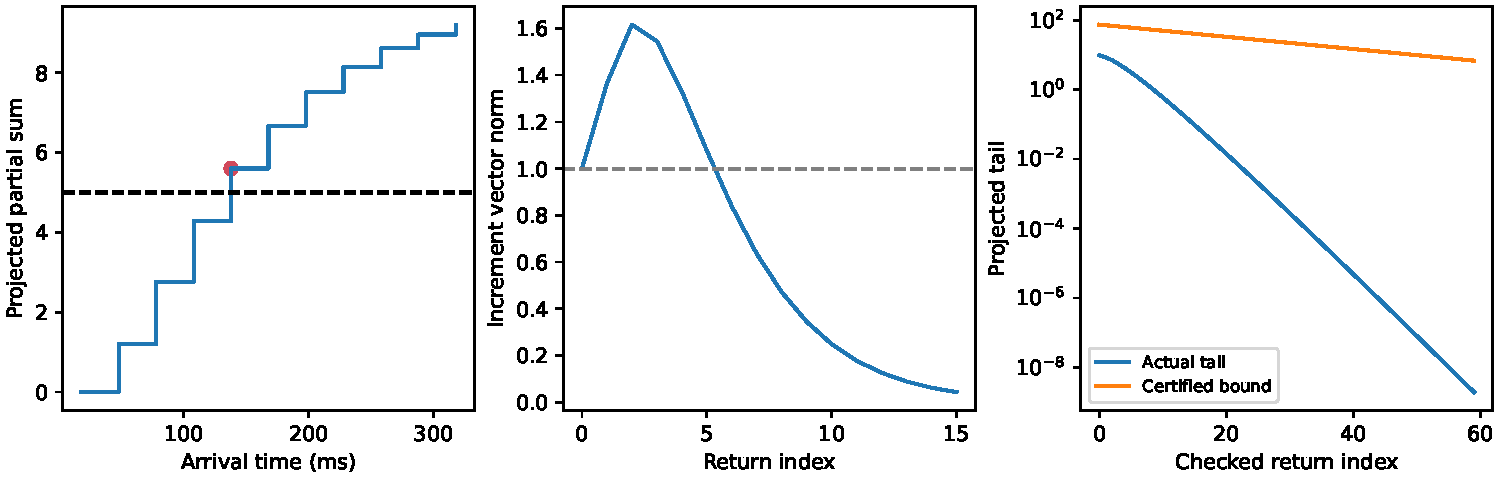
\includegraphics[width=.95\linewidth]{figure_nonnormal.pdf}\caption{Stable non-normal returns. Left: a zero direct readout crosses threshold 5 at the fourth return. Middle: individual increments can amplify in Euclidean norm although the spectral radius is 0.65. Right: the Lyapunov tail bound contains the actual projected tail and can be conservative. All values are synthetic.}\label{fig:supp-nonnormal}\end{figure}
\begin{figure}[H]\centering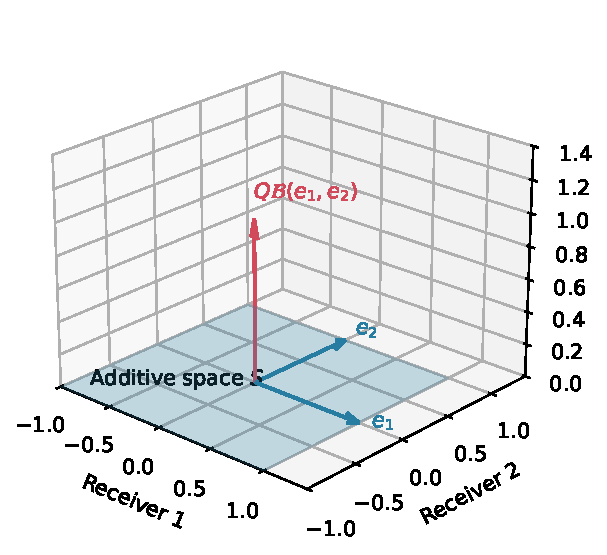
\includegraphics[width=.72\linewidth]{figure_innovation_geometry.pdf}\caption{Interaction geometry for the exact three-coordinate example: additive responses occupy $S=\operatorname{span}\{e_1,e_2\}$, while the bilinear product contributes along $e_3\in S^\perp$. The added rank is one across conditions; a class-independent product has zero class contrast despite this rank.}\end{figure}
For the gate $g(\delta)=\exp[-\kappa(1-\cos\delta)]$, $\kappa=0$ gives constant gain; finite positive $\kappa$ gives positive opposite-phase attenuation. A half-height angle exists when $\kappa\ge\log(2)/2$ and solves $\cos\delta_{1/2}=1-\log(2)/\kappa$. At smaller concentrations the gate stays above half height even at opposite phase. Estimate amplitude, center and concentration on independent calibration probes with matched input content, then freeze them. Unknown filter phase and upstream state changes can invalidate the biological interpretation. The example $\kappa=2$ is an illustrative concentration, not a measured universal neural value.

\section*{S18. Symbol glossary and model boundaries}
\begin{center}\small\begin{tabular}{@{}p{.25\linewidth}p{.67\linewidth}@{}}\toprule
Symbols & Meaning\\\midrule
$z,d,D_j,D_i,T_{ij},M$ & Anchored item; source perturbation; encoders; translation; composite translated encoder\\
$B_{ij}$ & Translation error $T_{ij}D_j-D_i$\\
$\Omega,\tau,\alpha,\gamma$ & Angular frequency; conduction; receptive center; carrier transfer phase\\
$\eta,\xi,\psi,\Delta$ & Gate offset; carrier offset; calibrated probe phase contrast; arrival error\\
$g,\kappa,r,w,H,h$ & Gate; concentration; gain; pathway weight; Fourier processing response; causal processing density\\
$a_v,A_v,\theta_{\rm comm}$ & Delivered item amplitude; its maximum over phase; operational threshold\\
$P,Q,L_{PQ},L_{QP}$ & Loop populations and forward/reverse content maps (first index is receiver)\\
$A,p_0,v,T_{\rm loop}$ & Return product; initial projected vector; readout; round-trip delay\\
$\mathcal S_d,z_m,E_m,G_A$ & Item Krylov space; scalar partial sum; tail bound; Lyapunov metric\\
$S_1,S_2,S,C_B,d_B$ & Pathway images; their sum; basis-product matrix; added innovation rank\\
$\mathcal B,k,\chi,U,V$ & Bilinear map; interaction memory; coefficient; translated inputs\\
$\Sigma,W,Q_\Sigma,\lambda$ & Readout covariance; whitening; complement projector; interaction gain\\
$T_n,T_*,u_n,v_n,G$ & Learned map; target; teaching input/target; weighted excitation\\
$\varepsilon,\ell_n,r_n$ & Learning step; opportunity flag; teaching gain\\\bottomrule
\end{tabular}\end{center}
Some symbols are local to distinct modules: $Q$ is a regional loop signal in the reciprocal model and an orthogonal projector in the interaction-rank proposition; $A$ is an access-set label in the introductory route example and a return-product matrix in the loop. Each is defined at its local first use. No equivalence between these objects is assumed.
The paper does not infer experience or report from projection, identify unconstrained processing phases, resolve all wrapped aliases, or validate a biological learning rule. Threshold completion, the readout likelihood, and the learning update are separately testable modeling assumptions. This glossary consolidates boundaries without changing any theorem's domain.
